\documentclass[conference]{IEEEtran}
\IEEEoverridecommandlockouts
% Paquetes para español
\usepackage[spanish]{babel}
\usepackage[utf8]{inputenc}
\usepackage{cite}
\usepackage{amsmath,amssymb,amsfonts}
\usepackage{algorithmic}
\usepackage{graphicx}
\usepackage{textcomp}
\usepackage{booktabs}
\usepackage{xcolor}
\usepackage{tikz}
\usetikzlibrary{calc}
% Si falta una imagen, muestra un recuadro en lugar de detener la compilación
\let\oldincludegraphics\includegraphics
\renewcommand{\includegraphics}[2][]{\IfFileExists{#2}{\oldincludegraphics[#1]{#2}}{\fbox{\parbox{0.8\columnwidth}{\centering Imagen faltante:\\ \texttt{\detokenize{#2}}}}}}
\def\BibTeX{{\rm B\kern-.05em{\sc i\kern-.025em b}\kern-.08em
    T\kern-.1667em\lower.7ex\hbox{E}\kern-.125emX}}
\begin{document}

\title{Red neuronal multicapa con retropropagación: clasificación del estado nutricional en cuatro categorías a partir de altura y peso}

\author{\IEEEauthorblockN{1\textsuperscript{st} Oscar Alberto Gallo García}
\IEEEauthorblockA{\textit{M. C. en Robótica e Inteligencia Artificial} \\
\textit{Centro Universitario de Ciencias Exactas e Ingenierías}\\
Guadalajara, México \\
oscar.gallo5770@alumnos.udg.mx}
}

\maketitle

\begin{abstract}
    Se implementó desde cero un perceptrón multicapa con una capa oculta,
    entrenado mediante el algoritmo de retropropagación del error en modalidad
    estocástica. La red se empleó para clasificar a adultos mexicanos de la
    ENSANUT 2022 en las cuatro categorías de la OMS, bajo peso, peso normal,
    sobrepeso y obesidad, utilizando únicamente su altura y su peso como
    entradas. El índice de masa corporal se utilizó exclusivamente para
    construir las etiquetas. Con una arquitectura 2--6--4, activación sigmoide
    logística en ambas capas y codificación \textit{one-hot}, la energía
    promedio del error descendió de $0.3246$ a $0.0266$ en $200$ épocas y la
    exactitud alcanzó $97.12\%$ en el conjunto de prueba. La red construyó
    regiones de decisión independientes para las clases peso normal,
    sobrepeso y obesidad, cuyos errores se concentran en las fronteras
    teóricas $m=25h^2$ y $m=30h^2$, superando la limitación de la frontera
    lineal única de ADALINE. No obstante, la clase bajo peso, que representa apenas el $1.4\%$
    de los datos, no fue reconocida por la red, lo cual evidencia el efecto
    del desbalance de clases sobre el criterio de error cuadrático.
\end{abstract}

\begin{IEEEkeywords}
Perceptrón multicapa, retropropagación, descenso de gradiente estocástico, clasificación multiclase, regiones de decisión, IMC
\end{IEEEkeywords}

\section{Introducción}
En la práctica anterior se estudió ADALINE, una neurona lineal cuyo
aprendizaje se formula como la minimización de una función de costo
cuadrática mediante descenso de gradiente. Dicho modelo solo es capaz de
representar una frontera lineal, por lo que su desempeño quedó limitado
por la curvatura de la frontera real $m=25h^2$ en el plano altura--peso.

El perceptrón multicapa generaliza esta idea al introducir una o más capas
ocultas con funciones de activación no lineales. La dificultad adicional
consiste en que los pesos de las capas ocultas influyen en el error de
manera indirecta. El algoritmo de retropropagación resuelve este problema
aplicando la regla de la cadena para atribuir a cada neurona un gradiente
local, el cual se propaga desde la capa de salida hacia las capas
anteriores \cite{b1,b2,b3,b4,b5}.

En esta práctica se conservan las cuatro categorías originales del IMC. Como
las fronteras ideales entre ellas son las parábolas
\begin{align}
    \label{eq:fronteras}
    m=18.5h^2,\qquad m=25h^2,\qquad m=30h^2,
\end{align}
con $h$ en metros y $m$ en kilogramos, el problema exige construir regiones
de decisión no lineales, lo que permite evaluar directamente la capacidad de
representación que aporta la capa oculta.

\section{Desarrollo}

\subsection{Base de datos}
Se utilizó la misma base de antropometría de la \textit{Encuesta Nacional de
Salud y Nutrición Continua 2022}, ENSANUT 2022, archivo
\texttt{ensaantro2022\_entrega\_w.csv}, publicada por el Instituto Nacional
de Salud Pública de México \cite{b6}. La base original contiene $15\,073$
registros y $98$ columnas, de las cuales se emplearon el peso
\texttt{an01\_1}, la estatura \texttt{an04\_1}, la edad \texttt{h0303} y la
condición de embarazo o lactancia \texttt{an06}.

Se aplicó exactamente la misma limpieza que en la Práctica~2, con el fin de
que los resultados de ambos modelos fueran comparables. Las columnas se
convirtieron a tipo numérico y se conservaron únicamente los registros que
cumplían simultáneamente las siguientes condiciones:
\begin{itemize}
    \item peso válido, $2\leq\text{peso}\leq250$ kg;
    \item estatura válida, $40\leq\text{estatura}\leq230$ cm;
    \item edad adulta, $20\leq\text{edad}\leq110$ años, ya que los puntos de
    corte del IMC de la OMS solo aplican a adultos;
    \item ausencia de embarazo y lactancia, $\texttt{an06}\notin\{1,2,3\}$.
\end{itemize}
La estatura se convirtió a metros. Tras la limpieza quedaron $N=6\,246$
registros, con alturas entre $1.065$ y $2.222$ m y pesos entre $32.05$ y
$222.22$ kg.

\subsection{Construcción de las cuatro clases}
Para cada registro se calculó el índice de masa corporal con las unidades
físicas originales,
\begin{align}
    \label{eq:imc}
    \text{IMC}(k)=\frac{\text{peso}(k)\,[\text{kg}]}{\left(\text{altura}(k)\,[\text{m}]\right)^2},
\end{align}
y se asignó una de las cuatro clases de la OMS:
\begin{align}
    \label{eq:clases}
    \begin{aligned}
    C_1&:\ \text{Bajo peso}, &&\text{IMC}<18.5,\\
    C_2&:\ \text{Peso normal}, &&18.5\leq\text{IMC}<25,\\
    C_3&:\ \text{Sobrepeso}, &&25\leq\text{IMC}<30,\\
    C_4&:\ \text{Obesidad}, &&\text{IMC}\geq30.
    \end{aligned}
\end{align}
El IMC se utilizó exclusivamente para generar la salida deseada y nunca
formó parte del vector de entrada, que se mantuvo como
$\mathbf{X}(k)=[\text{altura}(k),\ \text{peso}(k)]^\top$. El
Cuadro~\ref{tab:clases} y la Fig.~\ref{fig:hist} muestran un desbalance
severo: la clase $C_1$ contiene únicamente $85$ registros, es decir, el
$1.36\%$ del total, mientras que $C_3$ y $C_4$ concentran conjuntamente el
$78.1\%$.

\begin{table}[htbp]
\caption{Distribución de patrones por clase}
\label{tab:clases}
\begin{center}
\begin{tabular}{lrrrr}
\toprule
\textbf{Clase} & \textbf{Total} & \textbf{\%} & \textbf{Entren.} & \textbf{Prueba} \\
\midrule
$C_1$ Bajo peso   & $85$     & $1.36$  & $70$     & $15$  \\
$C_2$ Peso normal & $1\,286$ & $20.59$ & $1\,031$ & $255$ \\
$C_3$ Sobrepeso   & $2\,288$ & $36.63$ & $1\,834$ & $454$ \\
$C_4$ Obesidad    & $2\,587$ & $41.42$ & $2\,062$ & $525$ \\
\midrule
Total             & $6\,246$ & $100$   & $4\,997$ & $1\,249$ \\
\bottomrule
\end{tabular}
\end{center}
\end{table}

\begin{figure}[htbp]
\centering
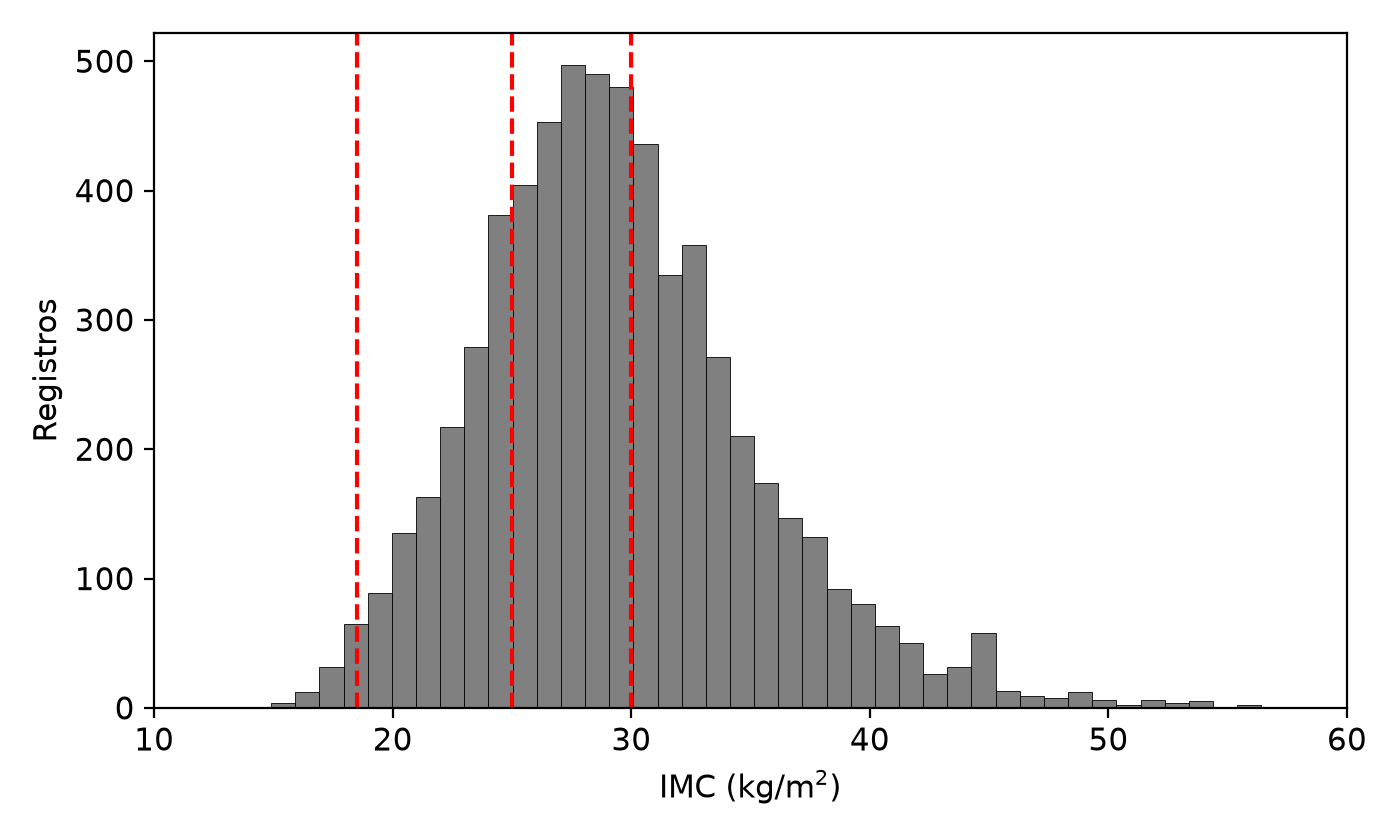
\includegraphics[width=\columnwidth]{figures/hist_imc4.png}
\caption{Histograma del IMC de los datos limpios. Las líneas punteadas
indican los umbrales $18.5$, $25$ y $30$ que separan las cuatro clases.}
\label{fig:hist}
\end{figure}

Las clases se representaron mediante codificación \textit{one-hot}, la cual
es consistente con el rango $[0,1]$ de la sigmoide logística empleada en la
capa de salida:
\begin{align}
    \label{eq:onehot}
    \begin{aligned}
    \mathbf{d}_{C_1}&=[1\ 0\ 0\ 0]^\top, &\mathbf{d}_{C_2}&=[0\ 1\ 0\ 0]^\top,\\
    \mathbf{d}_{C_3}&=[0\ 0\ 1\ 0]^\top, &\mathbf{d}_{C_4}&=[0\ 0\ 0\ 1]^\top.
    \end{aligned}
\end{align}

\subsection{Partición y escalamiento}
Se conservó la misma división de la Práctica~2: $80\%$ de los patrones para
entrenamiento, $4\,997$ en total, y $20\%$ para prueba, $1\,249$ en total,
mediante muestreo aleatorio con semilla fija \texttt{random\_state=42}. Las
proporciones de cada clase se mantienen prácticamente iguales en ambas
particiones, como se aprecia en el Cuadro~\ref{tab:clases}.

Las entradas se estandarizaron con
\begin{align}
    \label{eq:zscore}
    z_j(k)=\frac{x_j(k)-\mu_j}{\sigma_j},
\end{align}
con $\mu_1=1.5946$ m y $\sigma_1=0.1076$ m para la altura, y
$\mu_2=75.181$ kg y $\sigma_2=19.570$ kg para el peso, calculados
únicamente con los $4\,997$ patrones de entrenamiento. Se eligió la
estandarización porque en la práctica anterior demostró un
condicionamiento claramente superior al de la normalización Min--Max. Los
mismos parámetros se reutilizaron sin cambios para transformar el conjunto
de prueba y la malla del mapa de regiones de decisión.

\subsection{Arquitectura de la red}
La red implementada tiene la estructura 2--6--4: dos entradas, una capa
oculta con $N_h=6$ neuronas y cuatro neuronas de salida, una por clase
\cite{b1}. La Fig.~\ref{fig:arq} muestra la arquitectura y la notación
empleada, donde $w_{ji}^{(\ell)}$ conecta la neurona $i$ de la capa $\ell-1$
con la neurona $j$ de la capa $\ell$. El número total de parámetros libres
es $6\cdot2+6+4\cdot6+4=46$.

\begin{figure}[htbp]
\centering
\begin{tikzpicture}[x=1.9cm,y=0.72cm,
    neu/.style={circle,draw=blue!50!black,thick,minimum size=0.62cm,inner sep=0pt,font=\scriptsize},
    inp/.style={circle,draw=gray,fill=gray!15,minimum size=0.62cm,inner sep=0pt,font=\scriptsize},
    con/.style={-latex,gray!60,thin}]
  \foreach \i in {1,2} \node[inp] (x\i) at (0,{-1.5-2*(\i-1)}) {$x_{\i}$};
  \foreach \j in {1,...,6} \node[neu] (h\j) at (1,{-(\j-1)*1.0}) {$y^{(1)}_{\j}$};
  \foreach \j in {1,...,4} \node[neu] (o\j) at (2,{-0.75-(\j-1)*1.25}) {$y^{(2)}_{\j}$};
  \foreach \i in {1,2} \foreach \j in {1,...,6} \draw[con] (x\i) -- (h\j);
  \foreach \i in {1,...,6} \foreach \j in {1,...,4} \draw[con] (h\i) -- (o\j);
  \foreach \j/\c in {1/C_1,2/C_2,3/C_3,4/C_4} \node[font=\scriptsize,anchor=west] at ($(o\j)+(0.25,0)$) {$\c$};
  \node[font=\scriptsize] at (0,0.9) {Entrada};
  \node[font=\scriptsize] at (1,0.9) {Oculta $\ell=1$};
  \node[font=\scriptsize] at (2,0.9) {Salida $\ell=2$};
  \node[font=\scriptsize] at (0.5,-5.6) {$w^{(1)}_{ji},\ b^{(1)}_j$};
  \node[font=\scriptsize] at (1.5,-5.6) {$w^{(2)}_{ji},\ b^{(2)}_j$};
\end{tikzpicture}
\caption{Arquitectura 2--6--4 implementada. Ambas capas utilizan la
sigmoide logística como función de activación.}
\label{fig:arq}
\end{figure}

\subsection{Propagación hacia adelante}
Definiendo $y_i^{(0)}(k)=x_i(k)$, el potencial local y la salida de la
neurona $j$ en la capa $\ell\in\{1,2\}$ son
\begin{align}
    \label{eq:v}
    v_j^{(\ell)}(k)&=\sum_{i} w_{ji}^{(\ell)}(k)\,y_i^{(\ell-1)}(k)+b_j^{(\ell)}(k),\\
    \label{eq:y}
    y_j^{(\ell)}(k)&=\varphi\!\left(v_j^{(\ell)}(k)\right).
\end{align}
En forma matricial, que es como se programó, la propagación se expresa
como $\mathbf{y}^{(\ell)}=\varphi\!\left(\mathbf{W}^{(\ell)}\mathbf{y}^{(\ell-1)}+\mathbf{b}^{(\ell)}\right)$,
con $\mathbf{W}^{(1)}\in\mathbb{R}^{6\times2}$ y
$\mathbf{W}^{(2)}\in\mathbb{R}^{4\times6}$. En ambas capas se utilizó la
sigmoide logística con $a=1$, cuya derivada se programó explícitamente en
términos de su propia salida:
\begin{align}
    \label{eq:sigmoide}
    \varphi(v)=\frac{1}{1+e^{-v}},\qquad \varphi'(v)=\varphi(v)\left[1-\varphi(v)\right].
\end{align}
La clase predicha corresponde a la neurona de salida con mayor activación,
\begin{align}
    \label{eq:argmax}
    \hat{C}(k)=\arg\max_{j\in\{1,2,3,4\}} y_j^{(2)}(k).
\end{align}

\subsection{Función de error}
Para cada neurona de salida se define $e_j(k)=d_j(k)-y_j^{(2)}(k)$. La
energía instantánea del error y la energía promedio de una época son
\begin{align}
    \label{eq:E}
    E(k)=\frac{1}{2}\sum_{j=1}^{4}e_j^2(k),\qquad
    E_{\text{av}}=\frac{1}{N}\sum_{k=1}^{N}E(k).
\end{align}
La cantidad $E_{\text{av}}$ se registró al final de cada época y constituye
la curva de aprendizaje.

\subsection{Retropropagación}
Al aplicar la regla de la cadena, el gradiente local de una neurona de
salida resulta
\begin{align}
    \label{eq:delta2}
    \delta_j^{(2)}(k)=e_j(k)\,\varphi'\!\left(v_j^{(2)}(k)\right)
    =e_j(k)\,y_j^{(2)}(k)\left[1-y_j^{(2)}(k)\right].
\end{align}
Una neurona oculta carece de salida deseada; su contribución al error se
obtiene a través de las neuronas de la capa siguiente:
\begin{align}
    \label{eq:delta1}
    \delta_j^{(1)}(k)=y_j^{(1)}(k)\left[1-y_j^{(1)}(k)\right]\sum_{r=1}^{4}\delta_r^{(2)}(k)\,w_{rj}^{(2)}(k).
\end{align}
En forma matricial,
$\boldsymbol{\delta}^{(1)}=\left(\mathbf{W}^{(2)\top}\boldsymbol{\delta}^{(2)}\right)\odot\varphi'\!\left(\mathbf{v}^{(1)}\right)$.
Finalmente, todos los pesos y sesgos se actualizan con la regla general
\begin{align}
    \label{eq:updW}
    w_{ji}^{(\ell)}(k+1)&=w_{ji}^{(\ell)}(k)+\eta\,\delta_j^{(\ell)}(k)\,y_i^{(\ell-1)}(k),\\
    \label{eq:updb}
    b_j^{(\ell)}(k+1)&=b_j^{(\ell)}(k)+\eta\,\delta_j^{(\ell)}(k).
\end{align}
Los gradientes locales de ambas capas se calculan con los pesos vigentes
antes de modificar cualquier parámetro, de modo que la actualización es
coherente con el estado de la red para el patrón $k$.

\subsection{Parámetros de diseño}
El Cuadro~\ref{tab:diseno} resume la configuración utilizada. Se eligió la
modalidad estocástica, en la que los parámetros se actualizan
inmediatamente después de presentar cada patrón, lo que produce $N$
actualizaciones por época.

\begin{table}[htbp]
\caption{Parámetros de diseño de la red multicapa}
\label{tab:diseno}
\begin{center}
\begin{tabular}{ll}
\toprule
\textbf{Parámetro} & \textbf{Valor} \\
\midrule
Arquitectura         & 2--6--4, $46$ parámetros \\
Activación oculta    & Sigmoide logística, $a=1$ \\
Activación de salida & Sigmoide logística, $a=1$ \\
Codificación         & \textit{One-hot} en $\{0,1\}$ \\
Inicialización       & $w_{ji}^{(\ell)},b_j^{(\ell)}\sim\mathcal{U}(-1,1)$, semilla $42$ \\
Modalidad            & Estocástica, SGD, $M=1$ \\
Orden de patrones    & Fijo en todas las épocas \\
Razón de aprendizaje & $\eta=0.01$ \\
Épocas               & $200$ \\
Criterio de paro     & Número fijo de épocas \\
Escalamiento         & Estandarización, z-score \\
\bottomrule
\end{tabular}
\end{center}
\end{table}

El valor $N_h=6$ corresponde a una de las arquitecturas pequeñas sugeridas
en los lineamientos. Con tres fronteras curvas que separar, seis neuronas
ocultas proporcionan suficientes semiplanos sigmoidales para aproximar cada
parábola por tramos, sin incrementar en exceso el número de parámetros.

\subsection{Algoritmo}
El procedimiento se implementó en Python con NumPy, sin bibliotecas de redes
neuronales ni diferenciación automática:
\begin{algorithmic}[1]
\STATE Inicializar $\mathbf{W}^{(\ell)},\mathbf{b}^{(\ell)}\sim\mathcal{U}(-1,1)$
\FOR{$q=1$ \TO $200$}
    \STATE $S\leftarrow0$
    \FOR{cada patrón $k$}
        \STATE $\mathbf{y}^{(0)}\leftarrow\mathbf{z}(k)$
        \FOR{$\ell=1$ \TO $2$}
            \STATE $\mathbf{y}^{(\ell)}\leftarrow\varphi(\mathbf{W}^{(\ell)}\mathbf{y}^{(\ell-1)}+\mathbf{b}^{(\ell)})$
        \ENDFOR
        \STATE $\boldsymbol{\delta}^{(2)}\leftarrow(\mathbf{d}(k)-\mathbf{y}^{(2)})\odot\mathbf{y}^{(2)}\odot(1-\mathbf{y}^{(2)})$
        \STATE $\boldsymbol{\delta}^{(1)}\leftarrow(\mathbf{W}^{(2)\top}\boldsymbol{\delta}^{(2)})\odot\mathbf{y}^{(1)}\odot(1-\mathbf{y}^{(1)})$
        \FOR{$\ell=1$ \TO $2$}
            \STATE $\mathbf{W}^{(\ell)}\leftarrow\mathbf{W}^{(\ell)}+\eta\,\boldsymbol{\delta}^{(\ell)}\mathbf{y}^{(\ell-1)\top}$
            \STATE $\mathbf{b}^{(\ell)}\leftarrow\mathbf{b}^{(\ell)}+\eta\,\boldsymbol{\delta}^{(\ell)}$
        \ENDFOR
        \STATE $S\leftarrow S+\tfrac{1}{2}\|\mathbf{d}(k)-\mathbf{y}^{(2)}\|^2$
    \ENDFOR
    \STATE $E_{\text{av}}(q)\leftarrow S/N$
\ENDFOR
\STATE Clasificar el conjunto de prueba con \eqref{eq:argmax}
\end{algorithmic}

\section{Resultados}

\subsection{Curva de aprendizaje}
La energía promedio descendió de $E_{\text{av}}(1)=0.3246$ a
$E_{\text{av}}(200)=0.0266$, como se observa en la Fig.~\ref{fig:eav}. El
descenso fue rápido durante las primeras épocas, con
$E_{\text{av}}(10)=0.1481$, y posteriormente se volvió gradual, con
$E_{\text{av}}(50)=0.0433$ y $E_{\text{av}}(100)=0.0329$. La curva es
monótona y suave, sin indicios de divergencia ni de oscilaciones, lo cual
confirma que $\eta=0.01$ es adecuada para entradas estandarizadas. Al
concluir las $200$ épocas la curva aún presenta una pendiente ligeramente
negativa, por lo que un entrenamiento más prolongado podría reducir
marginalmente el error.

\begin{figure}[htbp]
\centering
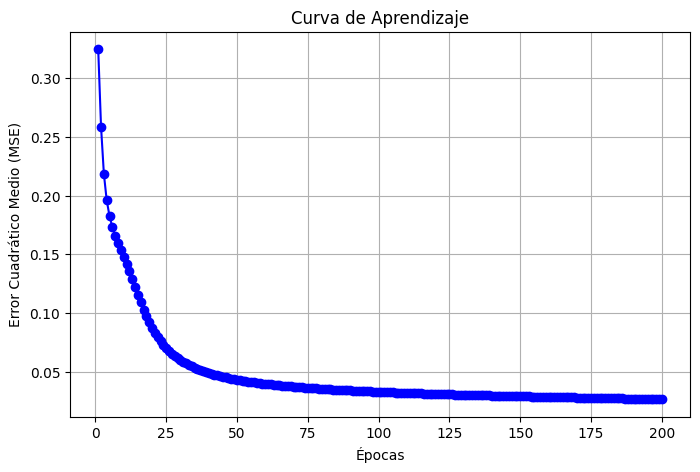
\includegraphics[width=\columnwidth]{figures/curva_eav.png}
\caption{Curva de aprendizaje de la red 2--6--4. El eje vertical, rotulado
como MSE, corresponde a la energía promedio del error $E_{\text{av}}$
definida en \eqref{eq:E}.}
\label{fig:eav}
\end{figure}

\subsection{Regiones de decisión}
Para construir el mapa de decisión se generó una malla regular de puntos,
con separación de $0.05$, sobre el espacio de entradas estandarizadas
$(z_1,z_2)$, que cubre el intervalo de los datos con un margen de $0.5$ en
cada eje. Cada punto se propagó por la red y se le asignó la clase con
\eqref{eq:argmax}. Las Figs.~\ref{fig:reg_test} y \ref{fig:reg_train}
muestran las regiones obtenidas junto con los patrones reales de prueba y
de entrenamiento, respectivamente. Los ejes corresponden a la altura y al
peso estandarizados, de modo que un punto de la gráfica se relaciona con
las unidades originales mediante $h=\mu_1+\sigma_1z_1$ y
$m=\mu_2+\sigma_2z_2$.

\begin{figure}[htbp]
\centering
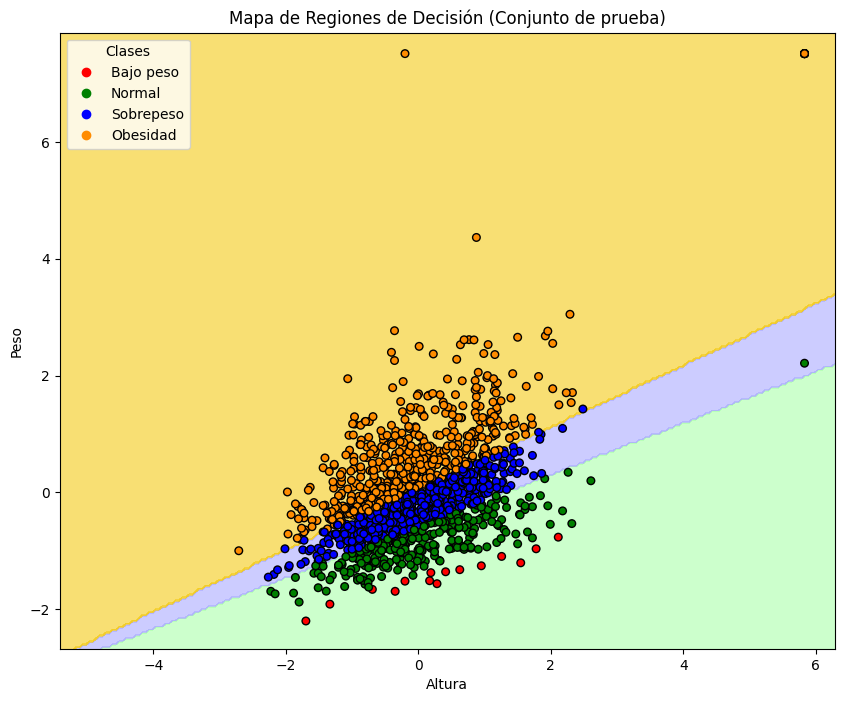
\includegraphics[width=\columnwidth]{figures/regiones_test.png}
\caption{Regiones de decisión de la red 2--6--4 en el espacio
estandarizado, con los patrones del conjunto de prueba.}
\label{fig:reg_test}
\end{figure}

\begin{figure}[htbp]
\centering
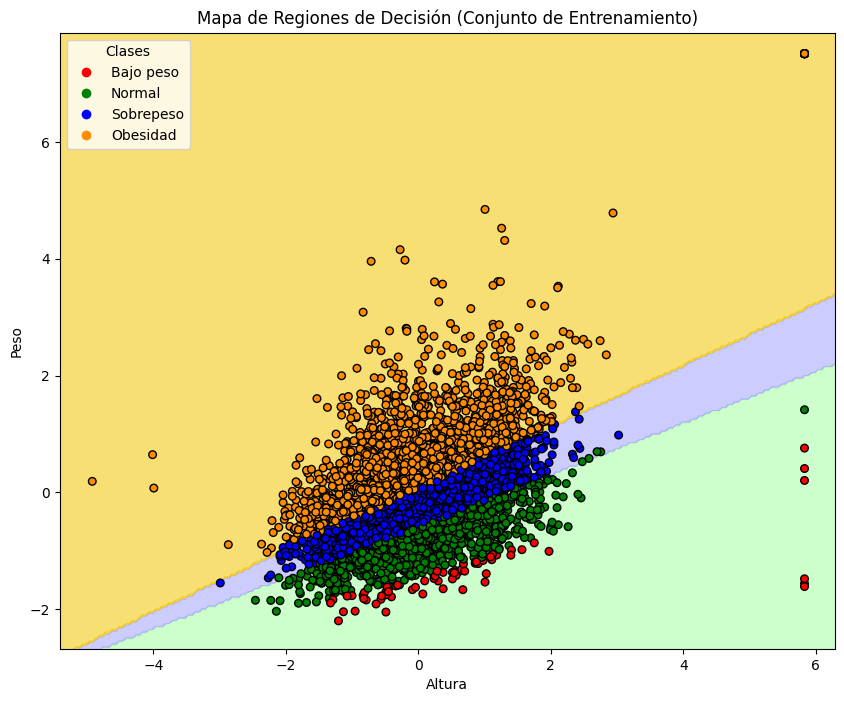
\includegraphics[width=\columnwidth]{figures/regiones_train.png}
\caption{Regiones de decisión de la red 2--6--4 en el espacio
estandarizado, con los patrones del conjunto de entrenamiento.}
\label{fig:reg_train}
\end{figure}

A diferencia de la única recta obtenida con ADALINE, la red construyó tres
regiones separadas por dos fronteras independientes: una entre peso normal
y sobrepeso y otra entre sobrepeso y obesidad. Ambas fronteras crecen con
la altura, lo cual es coherente con las fronteras teóricas
\eqref{eq:fronteras}, según las cuales el peso límite de cada categoría
aumenta con el cuadrado de la estatura. En la zona donde se concentran los
patrones, aproximadamente $-2\leq z_1\leq2$, las fronteras separan con
claridad las nubes de puntos de $C_2$, $C_3$ y $C_4$, y los patrones de
distinta clase solo se mezclan en las franjas contiguas a cada frontera.
Dentro de este intervalo la curvatura de las parábolas teóricas es pequeña,
por lo que las fronteras aprendidas resultan casi rectas. Fuera de él, donde
los datos son escasos, las fronteras se prolongan con pendiente
aproximadamente constante, ya que la red carece de información para
extrapolar la curvatura real. Por último, no se formó ninguna región para
$C_1$: los patrones de bajo peso, ubicados en la parte inferior de la nube,
quedaron dentro de la región asignada a $C_2$.

\subsection{Desempeño en entrenamiento y prueba}
El Cuadro~\ref{tab:desempeno} resume los resultados en ambos conjuntos. La
exactitud global fue de $97.52\%$ en entrenamiento y de $97.12\%$ en prueba,
\begin{align*}
    \text{Accuracy}_{\text{prueba}}=\frac{1\,213}{1\,249}\times100\%=97.12\%.
\end{align*}

\begin{table}[htbp]
\caption{Resultados en entrenamiento y prueba, red 2--6--4}
\label{tab:desempeno}
\begin{center}
\begin{tabular}{lrr}
\toprule
\textbf{Métrica} & \textbf{Entrenamiento} & \textbf{Prueba} \\
\midrule
Patrones               & $4\,997$  & $1\,249$ \\
Correctos              & $4\,873$  & $1\,213$ \\
Incorrectos            & $124$     & $36$ \\
Exactitud global       & $97.52\%$ & $97.12\%$ \\
\midrule
Acierto $C_1$ Bajo peso   & $0.00\%$  & $0.00\%$ \\
Acierto $C_2$ Peso normal & $98.64\%$ & $98.43\%$ \\
Acierto $C_3$ Sobrepeso   & $98.96\%$ & $97.36\%$ \\
Acierto $C_4$ Obesidad    & $98.98\%$ & $99.05\%$ \\
\bottomrule
\end{tabular}
\end{center}
\end{table}

La matriz de confusión del conjunto de prueba se presenta en el
Cuadro~\ref{tab:cm} y en la Fig.~\ref{fig:cm}. Todos los errores se
producen entre clases adyacentes, es decir, la red nunca confunde
categorías no contiguas, como peso normal con obesidad.

\begin{table}[htbp]
\caption{Matriz de confusión $4\times4$ en el conjunto de prueba}
\label{tab:cm}
\begin{center}
\begin{tabular}{c|cccc|r}
\toprule
 & $\hat{C}_1$ & $\hat{C}_2$ & $\hat{C}_3$ & $\hat{C}_4$ & \textbf{Acierto} \\
\midrule
$C_1$ & $0$ & $15$  & $0$   & $0$   & $0.00\%$ \\
$C_2$ & $0$ & $251$ & $4$   & $0$   & $98.43\%$ \\
$C_3$ & $0$ & $4$   & $442$ & $8$   & $97.36\%$ \\
$C_4$ & $0$ & $0$   & $5$   & $520$ & $99.05\%$ \\
\bottomrule
\end{tabular}
\end{center}
\end{table}

\begin{figure}[htbp]
\centering
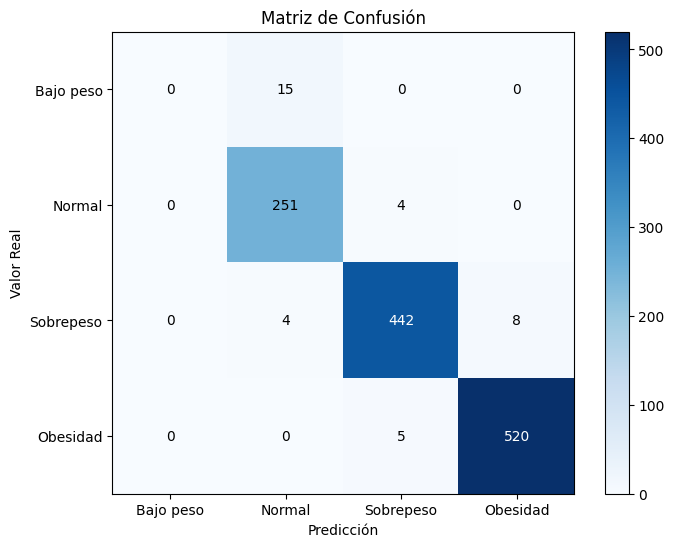
\includegraphics[width=0.85\columnwidth]{figures/matriz_confusion4.png}
\caption{Matriz de confusión de la red 2--6--4 en el conjunto de prueba.}
\label{fig:cm}
\end{figure}

\subsection{Análisis de errores}
Para cada patrón de prueba mal clasificado se calculó su distancia al
umbral de IMC más cercano. El Cuadro~\ref{tab:errores} muestra que los
errores se concentran fuertemente alrededor de las fronteras: $25$ de los
$36$ errores ocurren a menos de $0.5$ unidades de IMC de algún umbral, a
pesar de que esa banda contiene solo $177$ de los $1\,249$ patrones.

\begin{table}[htbp]
\caption{Errores de prueba según su distancia al umbral de IMC más cercano}
\label{tab:errores}
\begin{center}
\begin{tabular}{lccc}
\toprule
\textbf{Banda} & \textbf{Patrones} & \textbf{Errores} & \textbf{\% de errores} \\
\midrule
$<0.5$ & $177$ & $25$ & $69.4\%$ \\
$<1$   & $339$ & $31$ & $86.1\%$ \\
$<2$   & $703$ & $35$ & $97.2\%$ \\
\bottomrule
\end{tabular}
\end{center}
\end{table}

El Cuadro~\ref{tab:ejemplos} presenta ejemplos representativos. Los
errores entre $C_2$, $C_3$ y $C_4$ corresponden a patrones prácticamente
situados sobre la frontera, con IMC de $25.009$ o $29.995$, para los cuales
una diferencia de pocos gramos determina la categoría. Por el contrario,
los $15$ patrones de $C_1$ fueron asignados a $C_2$ independientemente de su
distancia al umbral, incluso con IMC de $16.08$. El único error alejado de
las fronteras corresponde a un registro de $2.222$ m y $118.45$ kg, valor de
estatura que coincide con el código de no respuesta $222.2$ cm que el filtro
de rango no eliminó.

\begin{table}[htbp]
\caption{Ejemplos de patrones de prueba mal clasificados}
\label{tab:ejemplos}
\begin{center}
\begin{tabular}{ccccc}
\toprule
$h$ [m] & $m$ [kg] & \textbf{IMC} & \textbf{Real} & \textbf{Predicha} \\
\midrule
$1.615$ & $48.25$  & $18.499$ & $C_1$ & $C_2$ \\
$1.412$ & $32.05$  & $16.075$ & $C_1$ & $C_2$ \\
$1.556$ & $60.55$  & $25.009$ & $C_3$ & $C_2$ \\
$1.721$ & $73.95$  & $24.968$ & $C_2$ & $C_3$ \\
$1.463$ & $64.20$  & $29.995$ & $C_3$ & $C_4$ \\
$1.530$ & $70.25$  & $30.010$ & $C_4$ & $C_3$ \\
$2.222$ & $118.45$ & $23.991$ & $C_2$ & $C_3$ \\
\bottomrule
\end{tabular}
\end{center}
\end{table}

\section{Discusión}

\textbf{Limitación de una neurona lineal.} Una sola neurona lineal divide el
plano altura--peso mediante una recta, mientras que las cuatro categorías
están delimitadas por tres parábolas \eqref{eq:fronteras}. Además, una
neurona produce una única salida y, por tanto, solo puede separar dos
regiones, de modo que resulta insuficiente tanto por la forma de las
fronteras como por el número de clases.

\textbf{Papel de la activación no lineal.} Cada neurona oculta define una
transición sigmoidal suave a lo largo de una dirección del plano. La capa de
salida combina estas transiciones, lo que permite construir fronteras
curvas por superposición. Si la activación oculta fuera lineal, la
composición de ambas capas seguiría siendo una transformación afín y la red
equivaldría a un clasificador lineal.

\textbf{Interpretación de los gradientes locales.} El término
$\delta_j^{(2)}(k)$ mide la sensibilidad del error con respecto al potencial
de la neurona de salida $j$: combina cuánto se equivocó la neurona, a
través de $e_j(k)$, con cuánto puede modificarse su salida, a través de
$\varphi'$. El término $\delta_j^{(1)}(k)$ representa la responsabilidad de
la neurona oculta $j$ en el error total; se obtiene sumando los errores de
salida ponderados por los pesos $w_{rj}^{(2)}$, ya que una neurona oculta
solo afecta al error a través de las conexiones que la unen con la capa
siguiente. Por ello, si dichos pesos son pequeños, el error retropropagado
hacia esa neurona también lo es.

\textbf{Entrenamiento frente a prueba.} La diferencia entre la exactitud de
entrenamiento, $97.52\%$, y la de prueba, $97.12\%$, es de apenas $0.40$
puntos porcentuales, y los aciertos por clase son muy similares en ambos
conjuntos. Dado que los patrones de prueba no intervinieron en el ajuste de
los pesos ni en el cálculo del escalamiento, esta diferencia constituye una
estimación válida de la capacidad de generalización e indica ausencia de
sobreajuste, lo cual es esperable con $46$ parámetros y casi $5\,000$
patrones.

\textbf{Ubicación de los errores.} Los errores se concentran sobre las
fronteras de IMC, como confirma el Cuadro~\ref{tab:errores}. Esto
demuestra que la red reprodujo adecuadamente las fronteras $m=25h^2$ y
$m=30h^2$, y que sus errores residuales se deben a la incertidumbre propia
de patrones casi equidistantes de dos clases. La excepción es la frontera
$m=18.5h^2$, que la red no aprendió.

\textbf{Efecto del desbalance de clases.} La clase $C_1$ cuenta con solo
$70$ patrones de entrenamiento, el $1.4\%$ del total. Como el entrenamiento
minimiza el error cuadrático promedio, la contribución de $C_1$ a
$E_{\text{av}}$ es marginal: asignar todos sus patrones a $C_2$ incrementa
poco el error global, mientras que crear una región específica para ellos
requeriría desplazar fronteras que afectan a miles de patrones de las
otras clases. En consecuencia, la exactitud global del $97.12\%$ oculta una
sensibilidad nula para $C_1$, lo que subraya la necesidad de reportar el
acierto por clase. Este comportamiento constituye un subajuste de la clase
minoritaria y podría mitigarse ponderando el error de cada clase de forma
inversamente proporcional a su frecuencia, sobremuestreando $C_1$ o
utilizando una salida \textit{softmax} con entropía cruzada.

\textbf{Efecto de la razón de aprendizaje.} Con $\eta$ demasiado pequeña la
red requiere muchas épocas para alcanzar la meseta del error y puede
quedar atrapada en zonas de saturación de la sigmoide, donde
$\varphi'\approx0$. Con $\eta$ demasiado grande las actualizaciones
estocásticas producen oscilaciones o incluso divergencia. El valor
$\eta=0.01$ produjo una curva monótona y estable.

\textbf{Parámetros de normalización.} Los parámetros $\mu_j$ y $\sigma_j$
forman parte del modelo y deben estimarse únicamente con los datos de
entrenamiento. Si se calculan con toda la base, la información del
conjunto de prueba se filtra al modelo y la evaluación deja de representar
el desempeño sobre datos verdaderamente nuevos.

\textbf{Comparación con ADALINE.} En el modelo se pasó de una neurona lineal
con una salida a una red con una capa oculta no lineal y cuatro salidas
sigmoidales. En el algoritmo de aprendizaje, la regla delta de ADALINE se
generalizó: la actualización conserva la forma
$\Delta w=\eta\,\delta\,y$, pero el término $\delta$ incorpora la derivada
de la activación y, en la capa oculta, se obtiene propagando hacia atrás
los gradientes locales de la salida. ADALINE alcanzó $88.39\%$ en un
problema de dos clases, mientras que la red multicapa logró $97.12\%$ en un
problema de cuatro clases.

\textbf{Limitaciones.}
\begin{itemize}
    \item El parámetro de mezcla de patrones se definió en la clase, pero
    no se aplicó, por lo que los patrones se presentaron en el mismo orden
    en todas las épocas.
    \item No se implementó un criterio de paro basado en el error; el
    entrenamiento se detuvo al completar $200$ épocas.
    \item La salida sigmoide con error cuadrático trata cada neurona de
    salida de forma independiente; una salida \textit{softmax}, cuya
    función se programó pero no se utilizó, produciría probabilidades
    normalizadas entre las cuatro clases.
    \item Persisten registros con los códigos de no respuesta $222.22$ kg y
    $222.2$ cm, que actúan como valores atípicos.
\end{itemize}

\section{Conclusiones}
Se implementó desde cero un perceptrón multicapa 2--6--4 entrenado con
retropropagación en modalidad estocástica, que alcanzó una exactitud de
$97.12\%$ al clasificar en cuatro categorías el estado nutricional de
adultos de la ENSANUT 2022 utilizando únicamente altura y peso. La curva de
aprendizaje fue monótona y estable, y la similitud entre los resultados de
entrenamiento y prueba indica una buena generalización.

La capa oculta permitió resolver lo que ADALINE no podía representar: la red
construyó varias fronteras de decisión independientes que separan con
claridad las clases peso normal, sobrepeso y obesidad, y los errores
residuales se localizan casi exclusivamente en las inmediaciones de las
fronteras teóricas $m=25h^2$ y $m=30h^2$. La principal deficiencia del modelo
es la nula detección de la clase bajo peso, consecuencia directa del
desbalance de clases bajo un criterio de error cuadrático. Como trabajo
futuro se propone incorporar ponderación por clase o sobremuestreo, emplear una salida
\textit{softmax} con entropía cruzada y añadir un criterio de paro basado en
un conjunto de validación.

\begin{thebibliography}{00}

\bibitem{b1} \textit{Algoritmo de retropropagación}, apuntes de clase del curso Sistemas Inteligentes 3 -- Redes Neuronales Artificiales, CUCEI, Universidad de Guadalajara, 2026.

\bibitem{b2} S. Haykin, \textit{Neural Networks and Learning Machines}, 3rd ed. Upper Saddle River, NJ, USA: Pearson/Prentice Hall, 2009.

\bibitem{b3} B. Mehlig, \textit{Machine Learning with Neural Networks: An Introduction for Scientists and Engineers}. Cambridge, U.K.: Cambridge University Press, 2021.

\bibitem{b4} C. C. Aggarwal, \textit{Neural Networks and Deep Learning: A Textbook}. Cham, Switzerland: Springer, 2018.

\bibitem{b5} I. Goodfellow, Y. Bengio, and A. Courville, \textit{Deep Learning}. Cambridge, MA, USA: MIT Press, 2016.

\bibitem{b6} Instituto Nacional de Salud Pública, ``Encuesta Nacional de Salud y Nutrición Continua 2022 (ENSANUT 2022): base de datos de antropometría,'' Cuernavaca, México: INSP, 2023. [En línea]. Disponible: https://ensanut.insp.mx

\end{thebibliography}

\end{document}
